\chapter{GTE: Spikes}
\label{sec:Spikes}
\ghnote{GH: Tekst nedenfor er sakset inn fra Gautes Sterratt-stoff. Maa omskrives for aa unngaa selv-plagiat. Tenker at vi ogsaa trenger en intro som bringer oss inn i stoffet.}

Extracellular potentials measured within neural tissue are often split into two separate frequency domains, which reflect different aspects of the underlying neural activity. The low frequency part, the local field potential (LFP), is thought to mostly reflect synaptic input to populations of pyramidal cells, while the high-frequency part, the multi-unit activity (MUA), reflects the population spiking activity (Fig.~\ref{XX:fig:LFP_MUA}).
%%%%%%%%%
% Figure
%%%%%%%%%
\begin{figure}[!ht]
\begin{center}
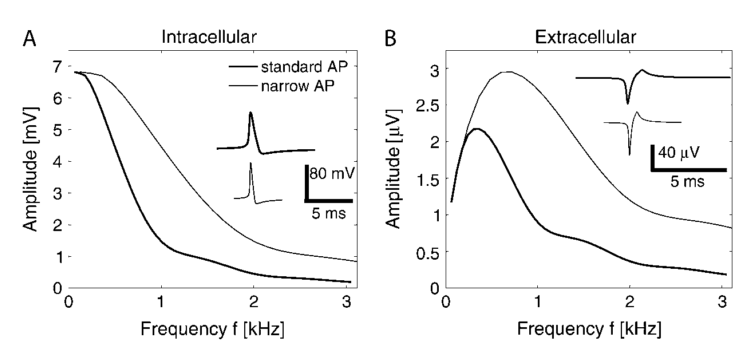
\includegraphics[width=0.6\textwidth]{Figures/Spikes/Spikes-eap_illustration.png}
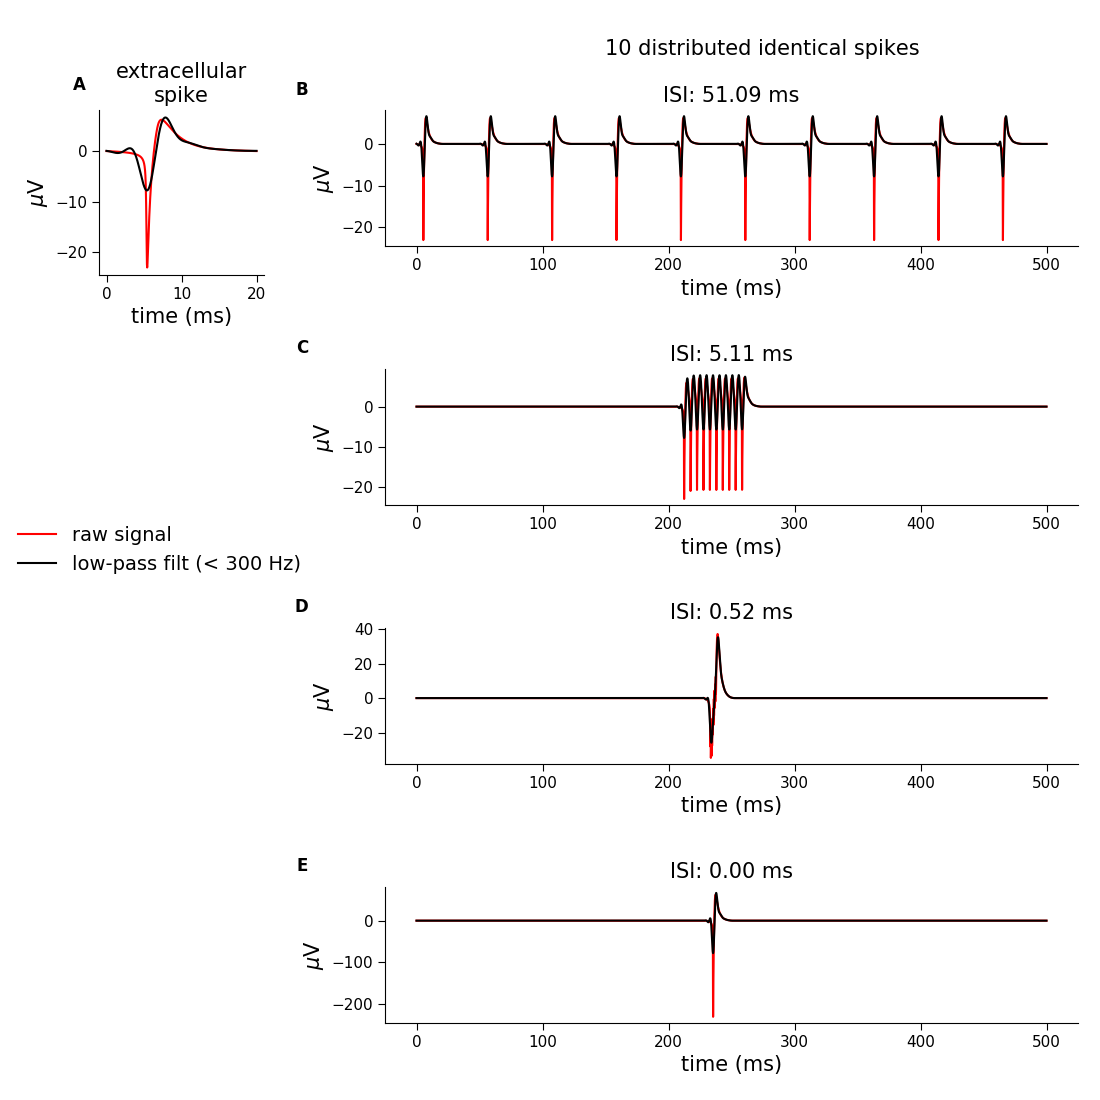
\includegraphics[width=0.6\textwidth]{Figures/Spikes/Spikes-LFP_spike_effect_test_300Hz.png}
\end{center}
\caption{\textbf{Potential EAP figures} 
Common misconception that spikes only have frequency content above a few hundred Hz. Delta pulse have flat frequency spectrum.}
\label{Spikes:fig:freq_dep}
\end{figure}

\section{\orange{Spikes in neurons with passive dendrites}}
\label{Spikes:sec:EP-spikes}
%Kjernereferanse: \cite**{Pettersen2008a}
%
%Perhaps start this by showing membrane potentials for cells with passive dendrites. 
%Then show extracellular signatures.


%%%%%%%%%%
% Figure: Intracellular and extracellular action potentials
%%%%%%%%%%
%\begin{cnfigure}{Figures/mm/EP-spike-Henze-w100-r150}
\begin{figure}[!ht]
\begin{center}
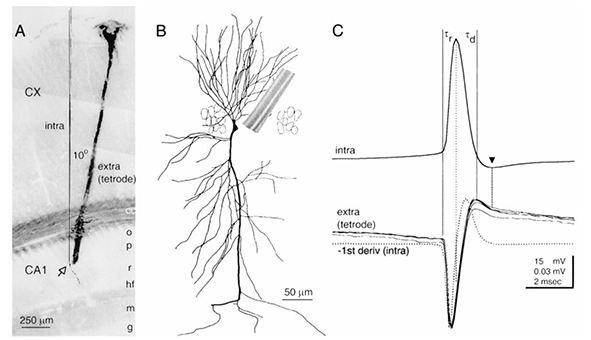
\includegraphics{Figures/Spikes/Spikes-Henze-w100-r150}
\end{center}
\caption[Intracellular and extracellular action potentials]{\textbf{Simultaneous recording of intracellular and extracellular action potentials (`spikes').}
Adapted from \citeasnoun**{Henze2000}.
\gen{Figure + caption to be updated}
}
\label{Spikes:fig:Henze}
\end{figure}
%%%%%%%%%%%


%The recording of spikes, the EPs corresponding to action potentials in individual neurons, has been
%key for learning about how neurons and neural networks function in live brains. 
When a sharp electrode is placed close to the soma of a neuron, an intracellular action potential will be seen
extracellularly as a sharp `spike' in the EP (Figure~\ref{Spikes:fig:Henze}). The magnitudes of these signals are quite different. While intracellular action potentials have amplitudes of $\sim$100~mV, the amplitudes of extracellular
spikes are typically less than 1~mV. Nevertheless, the detection of these spiking events from the recorded signal is relatively easily, and faithful records of the firing activity of neurons can be obtained. Such measurements have been instrumental in learning about \index{neural representations}, that is, how neurons in different parts of the brain, for example, encode information about visual and other sensory input. 

%%%
\subsection{\orange{Spikes from two-compartment neuron models}}
\label{Spikes:sec:EP-spikes-two-compartment}
%%%
Intracellular potentials can be modelled with a single-compartment neuron model as described in Chapter~3.
However, as described in the previous section, 
a two-compartment neuron model is the simplest model that can produce an extracellular potential such as a 
spike. An example of this is provided in Figure~\ref{Spikes:fig:TwoCompartment} where active sodium and potassium conductances are added to the  soma compartment of an otherwise passive neuron model. 
The membrane potential during a spike is illustrated in the right panel, and the  
corresponding EP is computed from Equation~\ref{XX:equation:Ve-two-compartment}. Around the soma a characteristic
EP spike with a sharp negative peak followed by a slower positive hump is seen, in accordance with typical experimental
spike recordings as exemplified by Figure~\ref{Spikes:fig:Henze}. Around the dendrite compartment inverted
spikes of the same sizes are seen, but such inverted spikes are rarely, if ever, seen in experiments. This suggests that
modelling dendrites as a single compartment is inadequate when one is interested in predicting the detailed spatial pattern of 
spike shapes that would be recorded by an electrode at different positions around a neuron.                                                                                                                                                                                                                                                                                                                                                                                                                                                                                                                                                                                                                                                                                                                                                                                                                                                                                                                                                                                                                                                                                                                                 

%%%%%%%%%%
% Figure: Spike from two-compartment model
%%%%%%%%%%
%\begin{cnfigure}{Figures/mm/EP-spike-TwoCompartment-w100-r150}
\begin{figure}[!ht]
\begin{center}
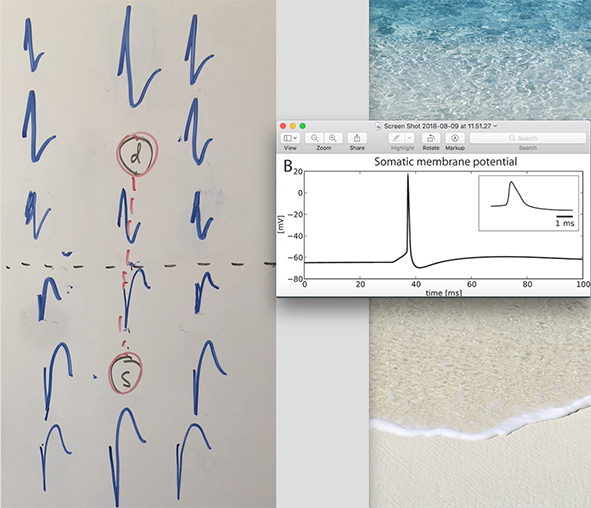
\includegraphics{Figures/Spikes/Spikes-TwoCompartment-w100-r150}
\end{center}
\caption{\textbf{EP (spike) from action potential for a two-compartment neuron model with active sodium
and potassium conductances in the soma compartment}. Computed from 
Equation~\ref{XX:equation:Ve-two-compartment}.
Left panel shows the EP at different spatial positions, while right panel shows the corresponding
soma membrane potential during the action potential. 
\gen{Figure + caption to be updated}
}
\label{Spikes:fig:TwoCompartment}
\end{figure}

%%%
\section{\orange{Spikes from multi-compartment neuron models}}
\label{Spikes:sec:EP-spikes-multi-compartment}
%%%
A more detailed picture of spike shapes is obtained by considering a detailed multi-compartmental neuron model
with a comprehensive branching structure typical for real neurons as in Figure~\ref{Spikes:fig:MultiCompartment}.
With this dendritic morphology the membrane currents through the dendrites are spread over a larger membrane area.
As a result, Equation~\ref{XX:equation:Ve-multi-compartment} predicts that the largest EP spikes will be seen
around the soma for the example pyramidal neuron in Figure~\ref{Spikes:fig:MultiCompartment}.  
Around the apical dendrites, the spikes will still have an inverted shape compared to spikes close to the soma. 
However, their amplitudes will be small, only a few microvolts, so they will not be seen in most experiments.

As for the two-compartment spike model, the spike amplitude in Figure~\ref{Spikes:fig:MultiCompartment} 
decays sharply with distance from the neuron. In addition, the spike width increases
with distance as demonstrated by the insets at two example positions. For the large spike recorded next to
the soma the half-width of the spike is $\sim$0.6~ms, while at the position outside the dendrite, the half-width is increased to
$\sim$0.7~ms. This corresponds to a low-pass filtering in the sense that the distant EP has lost some 
high-frequency components compared to the EP close to the soma. This filtering effect is absent for the spike generated by the 
two-compartment neuron model, and reflects that the cable properties of dendrites are important in determining 
also the shape of recorded spikes.   

%%%%%%%%%%
% Figure: Spike from multi-compartment model
%%%%%%%%%%
%\begin{cnfigure}{Figures/mm/EP-spike-MultiCompartment-w100-r150}
\begin{figure}[!ht]
\begin{center}
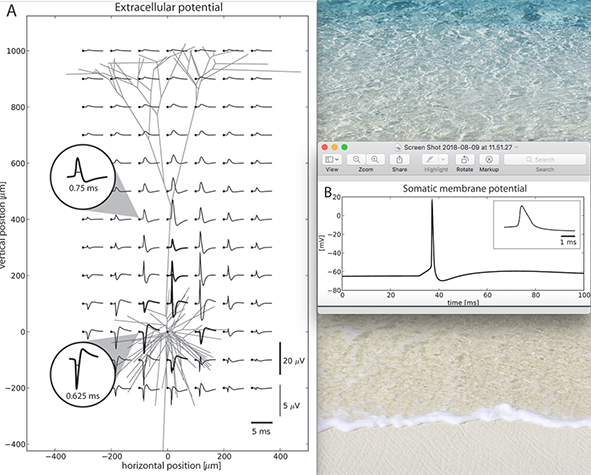
\includegraphics{Figures/Spikes/Spikes-MultiCompartment-w100-r150}
\end{center}
\caption[]{\textbf{EP (spike) from action potential for a multi-compartmental neuron model}. Active sodium
and potassium conductances in the soma compartment and computed from 
Equation~\ref{XX:equation:Ve-multi-compartment}.
Left panel shows the EP at different spatial positions, while right panel shows the corresponding
soma membrane potential during the action potential. 
\gen{Figure + caption to be updated. Change to Hay-model,}
}
\label{Spikes:fig:MultiCompartment}
%\figpermOurs
\end{figure}

%%%
\section{\orange{Spikes from ball-and-stick neurons}}
\label{Spikes:sec:spike-widths-amplitudes}
%%%
%\todo{June 2019: Make equivalent of old Figs. 12.6 for ball and stick?}
%%
The extracellular measurement of spikes from a neuron in living brains is blind in the sense that it is
unknown what type of neuron is recorded from when an electrode is lowered into the brain.
Some neuron types produce spikes with larger amplitudes and/or broader shapes than
others, and as seen in Figure~\ref{Spikes:fig:MultiCompartment} both the shape and amplitude 
depend critically on recording positions. Large spike amplitudes imply that they will be more dominant in electrical recordings,
and this bias should ideally be considered in the analysis of joint recordings 
of spikes from many neurons.

%%%%%%%
%% FIGURE - ball-and-stick spike
%%%%%%%
%\begin{figure}[t]
%  \multifigurebox{}{}{%
%    \vbox{%
%      \hspace*{8mm}\includegraphics{Figures/network/extracellular-arrangement}\\
%      \includegraphics{Figures/network/extracellular}}}
%  \caption{\emph{Simulation of \term{extracellular field potential}s. Extracellular
%    electrodes (black, grey, blue and dark-blue) are placed
%    close to a ball-and-stick model neuron with an active soma and
%    synapses on its dendrite. The soma is 40\uum long and 40\uum
%    in diameter. The single dendritic cable is 200\uum long and 4\uum in
%    diameter. The top traces show intracellular recordings when the
%    synapses are activated enough to cause an action potential to be
%    fired.  Traces are from the soma (black), halfway down the
%    dendrite (blue) and in the distal dendrite (dark-blue).
%    The initial synaptic stimulation can be seen in the dendritic
%    traces. The lower traces show the extracellular recordings
%    corresponding to the electrodes of the same colour.  During the
%    synaptic stimulation, the dendrites act as a sink of extracellular
%    current and the soma acts as a source. This can be seen in the
%    negative deflection of the extracellular potential in medial and
%    distal dendrites and the positive deflection of the extracellular
%    potential close to the soma. During the action potential, the soma
%    is a sink of current and the dendrites are current sources; this
%    is reflected in the large negative deflection of the extracellular
%    potential close to the soma and the smaller deflections of the
%    extracellular potential near the dendrites. As the neuron
%    repolarises, the roles of the soma and dendrites are again
%    reversed.} 
%        \gen{Revise: Figure and caption copied directly from first edition. Must be adapted.}}
%  %\figpermOurs
%  \label{mm:fig:extracellular}
%\end{figure}
%%%%%%%%%%%%%

 
To understand the link between the morphology of neurons and spikes amplitudes and shapes
it is convenient to consider ball-and-stick neurons where a dendrite cable `stick' is connected to a point-like soma.
%The relation between the intracellular action potential and the corresponding extracellular spike for such a 
%neuron is illustrated in the example in Figure~\ref{mm:fig:extracellular}.
Despite its simplicity, the ball-and-stick neuron model exhibits the key qualitative features observed in
Figure~\ref{Spikes:fig:MultiCompartment} 
when the multi-compartmental EP formula in  Equation~\ref{XX:equation:Ve-multi-compartment}
is used; that is, rapid attenuation of spike amplitude 
and increased spike width as the distance from the soma increases.
Figure~\ref{Spikes:fig:ball-and-stick-results}
shows the distance dependence of these spike measures both for a detailed multi-compartmental pyramidal neuron model 
and ball-and-stick neurons (Figure~\ref{Spikes:fig:ball-and-stick-neuron-models}).
While the spike width and amplitude of the multi-compartmental neuron are larger than for
the two example ball-and-stick neurons (with short and long dendrite sticks, respectively), 
the shapes of the curves are similar.\ghnote{GH: Kan vi ikke velge parametere slik at amplituden og shapen ligner i de to tilfellene?} Note also that the results for a ball-and-stick neuron with an infinitely long dendritic stick is
effectively identical to the long-stick results in the figure~\cite**{Pettersen2008}.
\gen{From David Sterratt: The frequency dependence here comes from intracellular properties? If so, would be great to make it clear.}


%%%%%%%%%%
% Figure: Neuron models considered in plot of spike widths and amplitudes
%%%%%%%%%% 
%\begin{cnfigure}{Figures/mm/EP-spike-ball-and-stick-neuron-models-w43-r300}
\begin{figure}[!ht]
\begin{center}
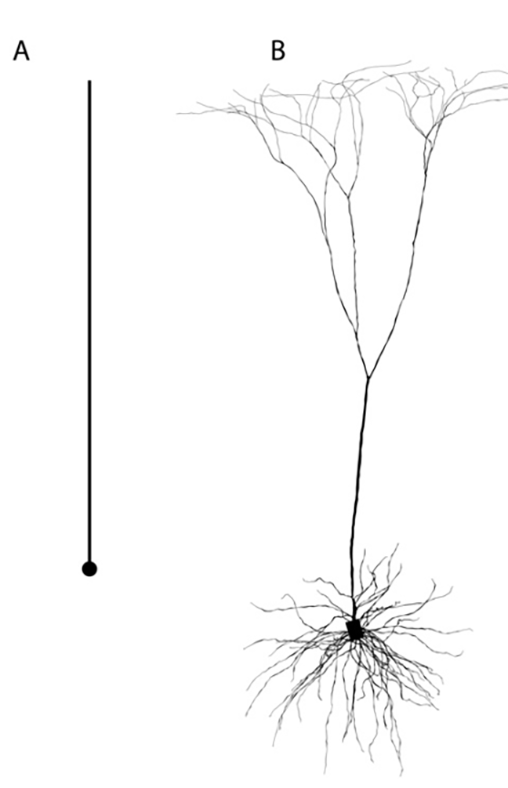
\includegraphics{Figures/Spikes/Spikes-ball-and-stick-neuron-models-w43-r300}
\end{center}
\caption[]{\textbf{Neuron models considered in results in Figure~\ref{Spikes:fig:ball-and-stick-results}}. 
\gen{Figure + caption to be updated.}
Adapted from \citeasnoun**{Pettersen2008}.
}
\label{Spikes:fig:ball-and-stick-neuron-models}
%\figpermOurs
\end{figure}

To understand the physical origin of these results it is easier to consider each frequency 
component of the action potential separately. From Fourier theory it follows that any signal
can be written of waves with different frequencies, so-called Fourier components (see sidebox).  
This is illustrated in Figure~\ref{Spikes:fig:ball-and-stick-frequency} where the weight of the different frequency components needed to
represent the intracellular action potential (membrane potential) and extracellular spike, respectively, are shown.
A key observation here is that for the extracellular spike, the largest
contributions comes from frequencies larger than 100~hertz.
\ghnote{Det overrasket at f-spektrum til intra vs ekstra er saa fundamentalt ulike. Er signalet i Figurpanel A ufiltrert, mens det i B er filtrert?}
%\todo{DCS: Ensure Figures/mm/dipole-comparison-w43-r300.png is committed
%  to git repository and then uncomment above line.}

For the ball-and-stick neuron, a membrane current entering the soma has to return to ECS through the cable stick, see Figure~\ref{Spikes:fig:ball-and-stick-sketch}. When an oscillating membrane current is entered through the soma, the spatial pattern of return current will depend on the frequency of the oscillation due to the capacitive properties of the membrane: For higher frequencies the capacitive membrane current will be larger, and the 
membrane effectively more leaky. Thus the injected soma current will return closer to the soma for higher frequencies, 
as  seen in the inset in Figure~\ref{Spikes:fig:ball-and-stick-sketch}.  


%%%%%%%%%%
% Figure: Action potential and its frequency content
%%%%%%%%%%
%\begin{cnfigure}{Figures/mm/EP-spike-ball-and-stick-frequency-w90-r150}
\begin{figure}[!ht]
\begin{center}
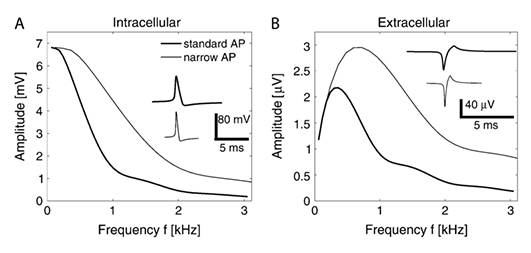
\includegraphics{Figures/Spikes/Spikes-ball-and-stick-frequency-w90-r150}
\end{center}
\caption[]{(a) Action potential used in simulations in Figure~\ref{Spikes:fig:ball-and-stick-results}(inset) 
and its frequency content.
%The intracellular spike width is defined as the
%width of the AP at half amplitude and is 0.55~ms for the standard
%AP, and half the value for the narrow AP. 
(b) Frequency content of example extracellular spike.
Inset: Typical spike shape computed a distance $r=10~\mu$m
perpendicular to the dendrite at the level of soma for a ball-and-stick 
neuron with diameter $d=2~\mu$m and infinite dendrite length.
Here the intracellular action potential in left panel was imposed as a voltage-clamp in the soma.
The extracellular spike width is defined as the width of the negative phase at 25\% of its maximum
amplitude and is 0.44~ms for the example spike.
The amplitude (peak-to-peak value) of the spike is $56~\mu$V  
\gen{Figure + caption to be updated. Will only include standard AP in final figure.} 
Adapted from \citeasnoun**{Pettersen2008}.}
\label{Spikes:fig:ball-and-stick-frequency}
%\figpermOurs
\end{figure}

To compute the EP generated by an imposed oscillatory current, the stick must be divided into small compartments  
and the multi-compartmental EP formula in Equation~\ref{XX:equation:Ve-multi-compartment} used. 
This in general requires detailed knowledge of the resulting membrane currents in all compartments. 
While these can be computed for the ball-and-stick neuron (see, for example, \citeasnoun**{Pettersen2014}), 
the resulting formula for the EP becomes cumbersome and difficult to interpret. 
However, as shown in XX
%Box~\ref{mm:box:ball-and-stick-spikes} 
some useful insights can be obtained in two limiting cases: the recording being very near to the soma or very far from the soma.

For recording positions very close to the soma, the contribution from the soma current will dominate 
in the sum in Equation~\ref{XX:equation:Ve-multi-compartment}. In this case the distance from the electrode
to the return currents in the dendrite will be much larger than the distance to soma. With only the contribution from
the soma compartment included, the amplitude $|\hat{V}_\mathrm{e,near}(f,\vec{r})|$  
of the EP signal for each Fourier component with frequency $f$ is found to be
%
\begin{equation}
  |\hat{V}_\mathrm{e,near}(f,\vec{r})| 
  \propto \frac{d^{3/2}}{r} \sqrt{ \frac{f C_\mathrm{m}}{R_\mathrm{a}} }  |\hat{V}_\mathrm{s}(f)| 
  \label{Spikes:equation:Ve_near}
\end{equation}
%
The suffix `near' is added because this expression only applies in the `near-field' limit, that is,
close to the soma.
$|\hat{V}_\mathrm{s}(f)|$ is the amplitude of Fourier component of the soma membrane potential at the same
frequency (see Figure~\ref{Spikes:fig:ball-and-stick-frequency}). Further, $d$ is the diameter of the dendritic
stick, $C_\mathrm{m}$ is the specific membrane capacitance, and $R_\mathrm{a}$ is the specific axial resistance.  
One of the predictions from the formula in Equation~\ref{Spikes:equation:Ve_near} is that the amplitude of each Fourier component decays
as $1/r$ when moving away from soma (yet staying within distances where the `near-field' approximation is still applicable).
Since this applies to all Fourier components which together constitute the action potential, this implies that the amplitude of the 
spike will decay as $1/r$ in this regime as well.
\gen{From David Sterratt: Intuition for the relationship witd $d, C_m, f, r_a$.}

For recording positions far away from the soma, the contribution from return membrane currents must be taken into
account in the sum in Equation~\ref{XX:equation:Ve-multi-compartment}. An approximate way of doing this is to
assume all return currents to leave the dendrite at a single point on the dendrite. Then we have 
a current dipole where the transmembrane current entering at the soma is balanced with a oppositely directed current
with the same magnitude leaving at a single point on the dendrite. The current dipole length is then given by the distance
between the soma and the dendritic position of the return current. An estimate of this length is provided by the 
frequency-dependent length constant  $\lambda_\mathrm{AC}(f)$  corresponding to the weighted mean of the positions of the return currents along
the dendrite stick (see Box XX). 
Then with the use of expression for the EP around a current dipole in 
Equation~\ref{XX:equation:Ve-dipole-p}:
%%%
\begin{equation}
  |\hat{V}_\mathrm{e,far}(f,\vec{r})|  \propto d^{2} \frac{|\cos \theta| }{r^2  R_\mathrm{a}}  |\hat{V}_\mathrm{s}(f)| 
  \label{Spikes:equation:Ve_far}
\end{equation}
%%%
The suffix `far' is addeds because this expression only applies in the `far-field' limit, that is,
far away from the soma. A first observation from this formula is that the EP is no longer radially symmetric, and depends both on the radial distance $r$ from the neuron and  the angle $\theta$ with the dipole axis, that is, the direction of the dendritic stick  (see Box~XX). The amplitude will be largest
above and below the neuron where $\theta=0^\circ$ and $\theta=180^\circ$, respectively. In the sideways direction 
($\theta \sim 90^\circ$) the EP will be much smaller, as is characteristic for spatial pattern of potentials around a current
dipole as illustrated in Figure~\ref{Spikes:fig:TwoCompartment}. A qualitatively similar dipolar pattern, although not so distinct,
is also seen for the spike generated by the biophysically detailed multi-compartment neuron in Figure~\ref{Spikes:fig:MultiCompartment}.

Another difference of this far-field expression with the near-field expression in Equation~\ref{Spikes:equation:Ve_near}, is that the
amplitude decays as $1/r^2$, characteristic for potentials around dipolar sources, rather than $1/r$ which is characteristic for potentials around 
a single source. This transition from a $1/r$ `monopolar' regime to a $1/r^2$ dipolar regime is indeed observed in
the spike-amplitude panel in Figure~\ref{Spikes:fig:ball-and-stick-results}.

There are several qualitative insights regarding the sizes and widths of spikes that can 
be found from the near-field and far-field formulae in Equations~\ref{Spikes:equation:Ve_near} and 
\ref{Spikes:equation:Ve_far}, respectively. One relates directly to the shape of the spike:
in the near-field expression, the high-frequency components of the spike is amplified 
compared to the low-frequency components, that is, $\hat{V}_\mathrm{e,near}(f,r) \propto \sqrt{f}$.
Thus close to the soma the spike is observed to be sharper than the intracellular action potential
as observed in the insets in Figure~\ref{Spikes:fig:ball-and-stick-frequency}. 
In the far-field regime there is no such high-frequency amplification ($\hat{V}_\mathrm{e,near}(f,r) \propto f^0 \sim 1$).
As a consequence, spikes measured far away from the soma will have less high-frequency content than those measured close to soma.
Thus the far-away spikes will be blunter and have larger spike widths as seen in the spike-width panel of 
Figure~\ref{Spikes:fig:ball-and-stick-results}.

The spike amplitude is proportional to $d^{2}$ far away from the soma and $d^{3/2}$ close to the soma,
where $d$ is the diameter of the dendritic stick diameter.
This implies that far-way from the soma the spike amplitude is proportional to the cross-sectional area of the dendrite.
Close to the soma, the spike amplitude also increases with dendrite diameter, but not so prominently as far away.
Another observation is that the spike amplitude is independent of the membrane resistance $R_\mathrm{m}$ of the dendrite; only the membrane 
capacitance $C_\mathrm{m}$ and the axial resistance $R_\mathrm{a}$ matter, 
This reflects that the frequencies dominating the spike are so high that the capacitive membrane current 
(governed by $C_\mathrm{m}$) is much larger than the ionic membrane current  (governed by $R_\mathrm{m}$). 
%\todo{DCS: I'm wondering if we need more details on frequency-dependent cable theory, beyond Eq. 5.11.}

An overall observation is that the spike is quite local, that is, the amplitude of the spike decays rapidly with distance from the neuron soma. For the pyramidal neuron considered in 
Figure~\ref{Spikes:fig:ball-and-stick-results}, for example, the spike amplitude decays from being about
300 microvolts a distance 20 micrometers from the soma center to being only about 10 microvolts a
distance 100 micrometers away. This rapid decay eases the interpretation of recorded spikes, since it implies
that in practice an electrode contact will only pick up spikes from neurons with somas positioned within a radius of some tens of micrometers.


%%%%%%%%%%
% Sidebox: Fourier sum
%%%%%%%%%%
%\begin{sidebox}
\subsection{\red{Side box: Fourier sum}}
\gen{This subsection used to be a side box in the Sterratt chapter}.
\ghnote{Appendix eller box?}
Time signals, such as the time course of a spike $V_\mathrm{e}(t)$,  can conveniently 
be represented as a sum of \index{Fourier components} with different frequencies $f$. 
Such a Fourier sum can be constructed in
various ways. The derivations in 
Section~\ref{Spikes:sec:spike-widths-amplitudes}, building on \citeasnoun**{Pettersen2008}, use the  
convention that a time signal $S(t)$ is the real part of the complex sum $\sum_{f}  \hat{S}(f) \exp (j 2 \pi f t)$. 
Here $j$ is the unit of imaginary numbers, and  $\hat{S}(f)$ is in general a complex number. 
%\end{sidebox}
%

%%%%%%%%%%
% Figure: Spike widths and amplitudes
%%%%%%%%%%
%\begin{cnfigure}{Figures/mm/EP-spike-ball-and-stick-results-w100-r150}
\begin{figure}[!ht]
\begin{center}
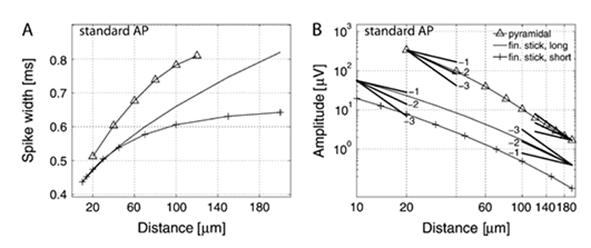
\includegraphics{Figures/Spikes/Spikes-ball-and-stick-results-w100-r150}
\end{center}
\caption[]{
Spike widths (left) and (peak-to-peak) spike amplitudes (right) as a function of
distance from soma for a detailed pyramidal cell model (pyramidal) and two
types of ball-and-stick models: long, finite ball-and-stick
model (fin.~stick, long) with diameter $d=2~\mu$m and length
$l=1$~mm and a short, finite ball-and-stick model (fin.~stick, short) with diameter $d=1~\mu$m and length $l=0.2$~mm,
see Figure~\ref{Spikes:fig:ball-and-stick-neuron-models}.
The intracellular action potential shown in the inset in the left panel of 
Figure~\ref{Spikes:fig:ball-and-stick-frequency} was imposed as a voltage-clamp in the soma.
The EP was recorded in the
somatic plane normal to the stick/primary apical dendrite. 
In right panels guidelines illustrating the power-law decays $1/r$ and
$1/r^{2}$ have been added. 
For further details see \citeasnoun[Figure 6]{Pettersen2008}.
\gen{Figure + caption to be updated.} 
Adapted from \citeasnoun**{Pettersen2008}.
}
\label{Spikes:fig:ball-and-stick-results}
%\figpermOurs
\end{figure}

%%%%%%%%%%
% Figure: Frequency-dependent distribution of return currents
%%%%%%%%%%
%\begin{cnfigure}{Figures/mm/EP-spike-ball-and-stick-sketch-w70-r300}
\begin{figure}[!ht]
\begin{center}
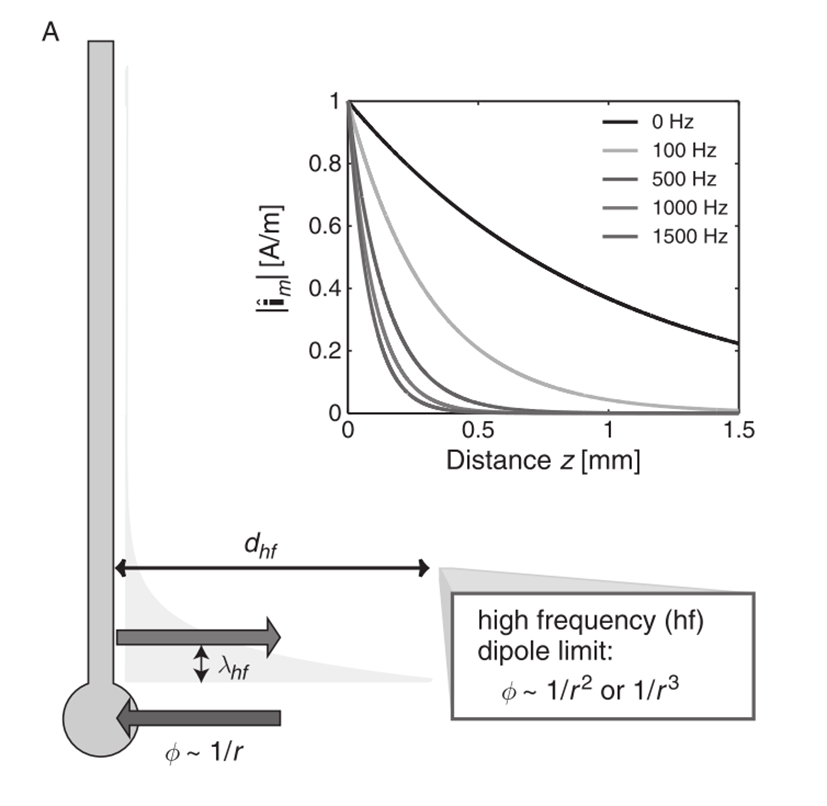
\includegraphics{Figures/Spikes/Spikes-ball-and-stick-sketch-w70-r300}
\end{center}
\caption[]{Illustration of ball-and-stick neuron and its frequency-dependent 
distribution of dendritic return currents following injection of a sinusoidal current into the soma.
The net current entering the soma will enter the dendrite as an axial current, and return to the 
ECS via the dendrite membrane. The inset shows the spatial distribution of this return current
for different frequencies. The higher the frequency, the closer the return currents will be and
the smaller the frequency-dependent length constant $\hat{\lambda}(f)$, reflecting the weighted mean 
of the return-current positions (see sidebox), will be. 
\gen{Figure + caption to be updated.} Adapted from \citeasnoun**{Pettersen2012}.
}
\label{Spikes:fig:ball-and-stick-sketch}
%\figpermOurs
\end{figure}
%

%%%%%%%%%%
% Box: Ball-and-stick model for spikes
%%%%%%%%%%
%\begin{boxfloat}{Ball-and-stick model for spikes}
%  \label{mm:box:ball-and-stick-spikes}  
\subsection{\red{Box: Ball-and-stick model for spikes}}
\gen{This was a box in the Sterratt chapter}
To understand the dependence of spike shapes and amplitudes on model parameters for the ball-and-stick neuron, it is useful
to consider the EP set up by each of the frequency (Fourier) components of the action potentials separately. 
For recording positions $\vec{r}$ very close to the soma, the contribution from the soma current will dominate over the contributions from the dendrite 
in the sum giving the EP in Equation~\ref{XX:equation:Ve-multi-compartment}. Then the amplitude of the
predicted oscillating EP $|\hat{V}_\mathrm{e,near}(f,\vec{r})|$ is approximately given by 
%
\begin{equation}
  |\hat{V}_\mathrm{e,near}(f,\vec{r})| = \frac{|\hat{I}_\mathrm{s}(f)|}{4 \pi \sigma r} 
  \label{Spikes:box:equation:Ve_near_1}
\end{equation}
%
where $|\hat{I}_\mathrm{s}(f)|$ is the amplitude of the oscillating current through the soma membrane.
%and also the axial current entering the dendrite from the soma compartment. 
For the relatively high frequencies of most relevance for the spike, this soma current is related to the soma membrane potential 
$\hat{V}_\mathrm{s}(f)$ through~\cite**{Pettersen2008}
%
\begin{equation}
  |\hat{I}_\mathrm{s}(f)| =  \frac{\pi^{3/2} d^{3/2}}{\sqrt{2}} \sqrt{ \frac{f C_\mathrm{m}}{R_\mathrm{a}} }  |\hat{V}_\mathrm{s}(f)|
  \label{Spikes:box:equation:Isoma}
\end{equation}
%
and the spike EP is thus found to be
%
\begin{equation}
  |\hat{V}_\mathrm{e,near}(f,\vec{r})| 
  = \frac{\sqrt{\pi}}{4 \sqrt{2} \sigma}
     \frac{d^{3/2}}{r} 
     \sqrt{ \frac{f C_\mathrm{m}}{R_\mathrm{a}} }  |\hat{V}_\mathrm{s}(f)| 
  \propto \frac{d^{3/2}}{r} \sqrt{ \frac{f C_\mathrm{m}}{R_\mathrm{a}} }  |\hat{V}_\mathrm{s}(f)| 
  \label{Spikes:box:equation:Ve_near_2}
\end{equation}
%
%
For recording positions further away from the soma, the contribution from return membrane currents must be taken into
account in the sum in Equation~\ref{XX:equation:Ve-multi-compartment}. An approximate way of doing this is to
assume all return currents to leave the dendrite at a single height $\lambda_\mathrm{AC}(f)$ above the soma, where 
this frequency-dependent length constant corresponds to the weighted mean of the positions of the return currents along
the dendrite stick. (The subscript `AC' denotes `alternating current'.)
Then the EP can be approximated by using the 
dipolar expression in Equation~\ref{XX:equation:Ve-dipole-p}, that is,
%%%
\begin{equation}
  |\hat{V}_\mathrm{e,far}(f,\vec{r})| =  \frac{|p(f) \cos \theta|}{4 \pi \sigma r^2} 
                                            = \frac{| \hat{I}_{s}(f) \lambda_\mathrm{AC}(f) \cos \theta|}{4 \pi \sigma r^2}   
                                                                                        \label{Spikes:box:equation:Ve_far_1}
\end{equation}
%%%
One way to define an AC length constant is as the mean value of the 
envelope of the sinusoidally varying (normalized) membrane current
$\hat{i}_\mathrm{m}$ weighted with distance $z$ from soma, 
see Figure~\ref{Spikes:fig:ball-and-stick-sketch}. 
For an infinite dendrite stick this corresponds to
%
\begin{equation}
  \lambda_\mathrm{AC}^\infty(f) = \frac{\int_0^\infty z |\hat{i}_\mathrm{m}| dz}{\int_0^\infty |\hat{i}_\mathrm{m}| dz} 
\nonumber
%=  \frac{\sqrt{2}\lambda}{\sqrt{\sqrt{W^2+1}+1}}.
\end{equation}
%

For high frequencies ($f \gg 1/2 \pi R_\mathrm{m} C_\mathrm{m}$) this is after some algebra 
found to give (see \citeasnoun[Appendix C]{Pettersen2008} for details)
%
\begin{equation}
 \lambda_\mathrm{AC}^\infty(f) =  \frac{\lambda}{\sqrt{\pi f \tau}} = 
  \frac{1}{2\sqrt{\pi}} \sqrt{\frac{d}{f R_\mathrm{m} C_\mathrm{m}}}
\label{Spikes:box:equation:approx_lambda_ac}
\end{equation}
%
where $\lambda$ is the cable length constant from 
%Chapter~\ref{XX:chap:XX}
Chapter~XX. 

%
Thus for EPs measured far away from the soma we find 
%  
\begin{equation}
  |\hat{V}_\mathrm{e,far}(f,\vec{r})|  = \frac{1}{8 \sqrt{2} \sigma} d^{2} \frac{1}{r^2  R_\mathrm{a}} 
      |\hat{V}_\mathrm{s}(f) \cos \theta | 
  \propto d^{2} \frac{|\cos \theta|}{r^2  R_\mathrm{a}} |\hat{V}_\mathrm{s}(f)| 
  \label{Spikes:box:equation:Ve_far_2}
\end{equation}
%
Equations~(\ref{Spikes:box:equation:Ve_near_2}) and (\ref{Spikes:box:equation:Ve_far_2}) describe how each frequency component of 
the soma membrane potential  $\hat{V}_\mathrm{s}(f)$ is `translated' into frequency components of the 
EP spike ($\hat{V}_\mathrm{e,near}(f,\vec{r})$ and $\hat{V}_\mathrm{e,far}(f,\vec{r})$, respectively). 
%\end{boxfloat}
%%%%%%%%%%%%%%%%%%%%%%%%%%%%%%%%%%%%%%%%%



%%%%%%%%%%
% Box: Spike sorting
%%%%%%%%%%
%\begin{boxfloat}{Spike sorting}
%  \label{mm:box:spike-sorting}
\subsection{\red{Box: Spike-sorting}}
\gen{This was a Box in the Sterratt chapter}
%
\centerline{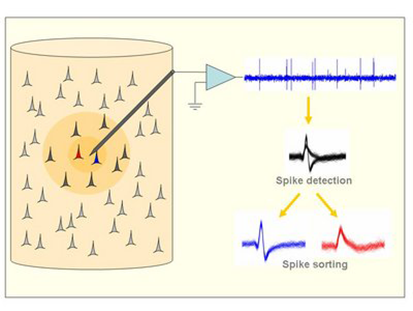
\includegraphics{Figures/Spikes/Spikes-sorting-w35-r300}}\vspace*{6pt}
%
A sharp electrode placed in brain tissue will pick up spiking signals from several neurons. 
However, the shapes of the spikes will be different for the different neurons, and this can be used to sort the spikes according to their neurons of origin. This is referred to as \index{spike sorting}, 
and is a problem of great practical importance both for neuroscience research and development of neuroprosthetic devices. 

In the present day with electrodes with hundreds or thousands of electrode recording contacts, fast and accurate automatic spike-sporting methods are needed to replace time-consuming manual spike-sorting methods~\cite**{Quiroga2007}. To develop and test such automatic methods, one needs
benchmarking spiking data where the `ground truth', that is, the actual spiking times for the contributing neurons, is known~\cite**{Einevoll2012}.
One use of the EP modelling scheme for spikes has been to generate such benchmarking data~\cite**{CamunasMesa2013,Hagen2015,MondragonGonzalez2017}. 

Modern electrodes have numerous recording contacts, often placed only some micrometers apart. Thus a spike can be measured at several contacts
simultaneously, each contact recording a slightly different shape reflecting the different positions of the contacts relative to the spiking neuron. 
This not only allows for accurate spike sorting, but also for estimation of the spatial position of the neuron. Likewise, the spatial variation of the 
spike shape around the neuronal soma (see Figure~\ref{Spikes:fig:MultiCompartment}) 
depends on the details of the intracellular action potential and dendritic morphology thus also allowing for the 
identification of neuron type~\cite**{Buccino2018}.    
\gen{Figure to be adapted from Quiroga (2007).}
%\end{boxfloat}
%%%


%%%%%%%%%%%%%%%%%%%%%%%%%%
% Box: Spike i MEA
%%%%%%%%%%    
\subsection{\red{Box:Spikes in microelectrode arrays (MEAs)}}
\gen{This was a box in Sterratt book chapter}
%\begin{boxfloat}{Spikes in microelectrode arrays (MEAs)}
%  \label{mm:box:spike-MEA}
As an alternative to measuring spikes in living brains, small slices of brain tissue can be put in suitably arranged dishes
where electrophysiological cellular properties can be studied for a few hours. Such \index{\emph{in vitro}} recordings
allows for more detailed and better controlled investigations than what can be achieved in living brains. In one type of such recordings
the brain tissue is placed on a \index{micro-electrode array (MEA)}. Here the bottom of the device contains a grid of electrode
contacts picking up electrical potentials generated by the neural activity of the slice of  brain tissue placed on top of it. 
The slice and the MEA are further covered with a liquid, typically saline, to keep the cells in the brain tissue functioning for the duration
of the experiment,  see figure:
%
\begin{center}
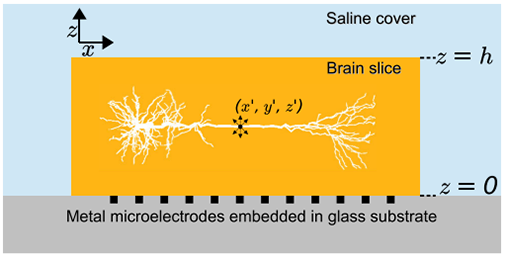
\includegraphics{Figures/Spikes/Spikes-MEA-1-w43-r300}
\end{center}
\vspace*{6pt}
%
In such measurements, the experimental set-up itself has an effect on recorded spikes. The microelectrode contacts are 
embedded in an insulating glass plate with very low electrical conductivity, while the saline has
a higher electrical conductivity than the brain slice it covers. 
For such planar step-wise discontinuities in the conductivity (assuming for the moment the MEA substrate, slice and saline
all are infinite planes) formulae analogous to Equation~\ref{XX:equation:Vr} can be derived by use of the
\index{method of images} from electrostatics, see Box~\ref{XX:box:MOI}.

While the largest effect on the recorded spike shape comes from the insulating 
glass substrate which roughly doubles the size of the recorded spikes, the figure below illustrates the 
effect from the saline covering the brain slice. As seen in the example results, the highly-conductive 
saline cover reduces the size of the recorded spike compared to the hypothetical 
situation where the saline had the same value of the electrical conductivity as the brain slice.
Figure is adapted from \citeasnoun**{Ness2015}.
%
\begin{center}
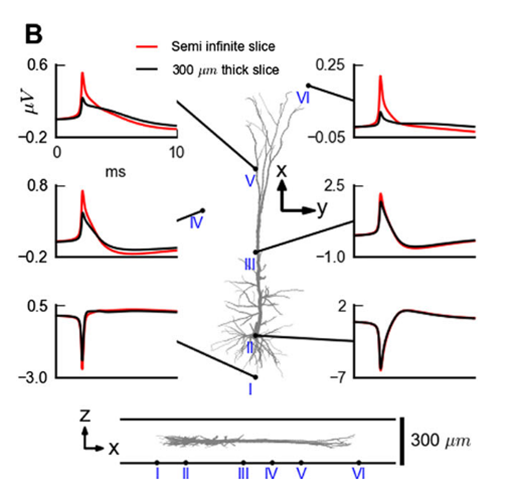
\includegraphics{Figures/Spikes/Spikes-MEA-2-w43-r300}
\end{center}
%
%\todo{DW: Too small.}
%\end{boxfloat}
%%%%%%%%%%%%%%%%%%%%%%%%%%%%%%%


While the formulae above were derived for a neuron model with a single passive dendritic stick, similar expressions can be derived for 
more complicated neuron models where several passive sticks protrude from the soma, see \citeasnoun**{Pettersen2008}.
The main conclusions above hold also for these neuron models, in particular that spike widths always increase with distance and that
the amplitude of a spike is proportional to $d^{k}$ where $k\sim1.5-2$. For neurons with many dendrites attached to the 
soma, the contributions to the spike amplitude roughly adds up. A simple rule of thumb is that a neuron's spike amplitude is 
roughly proportional to the sum of the cross-sectional areas for all dendrite branches attached directly onto to the soma. Neurons with many thick
dendritic branches attached to the soma will thus generate the largest spikes. See~\citeasnoun**{Pettersen2008} for further discussion.


{\bf TEXT COPIED FROM STERRATT CHAPTER ON 2020-10-13}

\section{Dependence of spike size and shape on neuronal properties}

Extracellular measurement of spikes from a neuron in living brains is blind in the sense that it is
not known what type of neuron is recorded from when an electrode is lowered into the brain.
Some neuron types produce spikes with larger amplitudes and/or broader shapes than
others,
%
%\todo{TVN: Nevne at det ofte sorteres i "putative excitatory" og "putative inhibitory"?}
%
and as seen in Figure~\ref{mm:fig:EP-spike-MultiCompartment} both the shape and amplitude 
depend critically on recording positions. Large spike amplitudes imply that they will be more dominant in electrical recordings,
and ideally this bias should  be considered in the analysis of joint recordings 
of spikes from many neurons. 

To understand the link between the morphology of neurons and their spike amplitudes and shapes
it is convenient to consider ball-and-stick neurons where a passive dendrite cable `stick' is connected to a point-like soma.
Despite its simplicity, the ball-and-stick neuron model exhibits the key qualitative features observed in
Figure~\ref{mm:fig:EP-spike-MultiCompartment} when the multi-compartmental EP formula in 
Equation~\ref{mm:equation:Ve-multi-compartment}
is used; that is, rapid attenuation of spike amplitude and increased spike width as the distance from the soma 
increases \cite**{Pettersen2008,Pettersen2012}. 

\citeasnoun**{Pettersen2008} took advantage of the mathematical tractability of the ball-and-stick model to
derive analytical expressions for how the amplitude of the recorded spike depends on distance from the neuron as well
as the electric properties of the neuron. The action potentials were decomposed into contributions from
many frequency components and each frequency component was considered individually.
This is illustrated in Figure~\ref{mm:fig:EP-spike-ball-and-stick-frequency} where the amplitudes of the different frequency components needed to
represent the intracellular action potential (membrane potential) and extracellular spike respectively are shown.
A key observation here is that for the extracellular spike, the largest contributions comes from frequencies larger than 100~hertz.
%%%%%%%%%%
% Figure: Action potential and its frequency content
%%%%%%%%%%
%\begin{cnfigure}{Figures/fig-not-pushed-to-github}
%\begin{cnfigure}{Figures/mm/EP-spike-ball-and-stick-frequency-w90-r150}
%\caption[]{
%Frequency content of example intracellular (a) and extracellular spike (b).
%%
%%(a) Action potential used in simulations in Figure~\ref{mm:fig:EP-spike-ball-and-stick-results}(inset) 
%%\todo{Comment from DCS not understood.}
%%and its frequency content. 
%%%The intracellular spike width is defined as the
%%%width of the AP at half amplitude and is 0.55~ms for the standard
%%%AP, and half the value for the narrow AP. 
%%(b) Frequency content of example extracellular spike.
%%Inset: Typical spike shape computed a distance $r=10~\mu$m
%%perpendicular to the dendrite at the level of soma for a ball-and-stick 
%%neuron with diameter $d=2~\mu$m and infinite dendrite length.
%%Here the intracellular action potential in left panel was imposed as a voltage-clamp in the soma.
%%The extracellular spike width is defined as the width of the negative phase at 25\% of its maximum
%%amplitude and is 0.44~ms for the example spike.
%%The amplitude (peak-to-peak value) of the spike is $56~\mu$V  
%\todo{Figure + caption to be updated. Will only include standard AP in final figure.} 
%Adapted from \citeasnoun**{Pettersen2008}.
%}
%\label{mm:fig:EP-spike-ball-and-stick-frequency}
%\figpermOurs
%\end{cnfigure}


%\todo{Explain the idea that the question is about how currents entering the soma during the AP returns through the dendrite}

\citeasnoun**{Pettersen2008} derived simple formulae relating the intracellular action potential to the extracellular spike for two limiting cases:
when the recording is done near to the soma or far away from the soma. For recordings near the soma the 
amplitude $|\hat{V}_\mathrm{e,near}(f,\vec{r})|$ of the spike signal for each frequency component with frequency $f$ was found to be approximated
by
%
\begin{equation}
  |\hat{V}_\mathrm{e,near}(f,\vec{r})| 
  \propto \frac{d^{3/2}}{r} \sqrt{ \frac{f C_\mathrm{m}}{R_\mathrm{a}} }  |\hat{V}_\mathrm{s}(f)| 
  \label{mm:equation:Ve_near}
\end{equation}
%
Here $|\hat{V}_\mathrm{s}(f)|$ is the amplitude of frequency component of the soma membrane potential at the same
frequency (see Figure~\ref{mm:fig:EP-spike-ball-and-stick-frequency}).
For recording positions far away from the soma, the following expression was instead found:
%%%
\begin{equation}
  |\hat{V}_\mathrm{e,far}(f,\vec{r})|  \propto d^{2} \frac{|\cos \theta| }{r^2  R_\mathrm{a}}  |\hat{V}_\mathrm{s}(f)| 
  \label{mm:equation:Ve_far}
\end{equation}
%%%
In these formulas, $d$ is the diameter of the dendritic
stick, $C_\mathrm{m}$ the specific membrane capacitance, and $R_\mathrm{a}$ the specific axial resistance.  


%%%%%%%%%%%
%% Figure: Spike widths and amplitudes
%%%%%%%%%%%
%\begin{cnfigure}{Figures/mm/EP-spike-ball-and-stick-results-w100-r150}
%\caption[]{
%Spike widths (left) and (peak-to-peak) spike amplitudes (right) as a function of
%distance from soma for a detailed pyramidal cell model (pyramidal) and two
%types of ball-and-stick models: long, finite ball-and-stick
%model (fin.~stick, long) with diameter $d=2~\mu$m and length
%$l=1$~mm and a short, finite ball-and-stick model (fin.~stick, short) with diameter $d=1~\mu$m and length $l=0.2$~mm,
%see Figure~\ref{mm:fig:EP-spike-ball-and-stick-neuron-models}.
%The intracellular action potential shown in the inset in the left panel of 
%Figure~\ref{mm:fig:EP-spike-ball-and-stick-frequency} was imposed as a voltage-clamp in the soma.
%The EP was recorded in the
%somatic plane normal to the stick/primary apical dendrite. 
%In right panels guidelines illustrating the power-law decays $1/r$ and
%$1/r^{2}$ have been added. 
%For further details see \citeasnoun[Figure 6]{Pettersen2008}.
%\todo{Figure + caption to be updated. Adapted from \citeasnoun**{Pettersen2008}.}
%}
%\label{mm:fig:EP-spike-ball-and-stick-results}
%\figpermOurs
%\end{cnfigure}


%\paragraph{Spike amplitude dependence on distance}
\subsection{Spike amplitude dependence on distance}
A prediction from the near-field formula in Equation~\ref{mm:equation:Ve_near} is that the amplitude of each Fourier component decays
as $1/r$ when moving away from the soma, whilst staying within distances where the `near-field' approximation still applies.
Since this applies to all frequency components which together constitute the action potential, this implies that the amplitude of the 
spike will decay as $1/r$ in this regime as well. 
Far away. the far-field formula (Equation~\ref{mm:equation:Ve_far}) implies that the spike amplitude depends not only depend on the radial distance $r$ from the neuron,
but also the angle $\theta$ with the dipole axis, the direction of the dendritic stick. The amplitude will be largest
above and below the neuron where $\theta=0^\circ$ and $\theta=180^\circ$, respectively. In the sideways direction 
($\theta \sim 90^\circ$) the spike will be much smaller, as is characteristic for spatial pattern of potentials around a current
dipole as illustrated in Figure~\ref{mm:fig:EP-spike-TwoCompartment}. A qualitatively similar dipolar pattern, although not so distinct,
is also seen for the spike generated by the biophysically detailed multi-compartment neuron in Figure~\ref{mm:fig:EP-spike-MultiCompartment}.
Another difference of this far-field expression with the near-field expression in Equation~\ref{mm:equation:Ve_near}, is that the
amplitude decays as $1/r^2$, characteristic for potentials around dipolar sources, rather than $1/r$ which is characteristic for potentials around 
a single source. %This transition from a $1/r$ `monopolar' regime to a $1/r^2$ dipolar regime was also found in model studies with biophysically detailed 
%neurons \cite[Fig.~X]{Pettersen2008}.
%\todo{Connect to Figure :EP-spike-ball-and-stick-results}

An overall observation is that the spike is quite local, with the amplitude of the spike decaying rapidly with distance from the neuron soma. 
For the pyramidal neuron considered in Figure~XX, for example, the spike amplitude decays from about
300 microvolts a distance 20 micrometers from the soma centre to only about 10 microvolts a
distance 100 micrometers away. 
%
%\todo{TVN:
%Kanskje fint med runde tall, men tror ofte man ikke "bruker" spikes med amplitude mindre enn ~30 muV, s{\aa} kunne kanskje valgt en kortere avstand for {\aa} ikke gi inntrykk av at man egentlig kan m{\aa}le spikes 100 mum fra soma?
%}
%
This rapid decay eases the interpretation of recorded spikes, since it implies
that in practice an electrode contact will only pick up spikes from neurons with somas positioned within a radius of some tens of micrometers.
%\todo{GTE: Rewrite this to compare with our own figure spikes around multicompartmental model + refer to Pettersen2008}  

%\paragraph{Spike amplitude dependence on neuronal parameters}
\subsection{Spike amplitude dependence on neuronal parameters}
The spike amplitude is proportional to $d^{2}$ far away from the soma and to $d^{3/2}$ close to the soma,
where $d$ is the diameter of the dendritic stick diameter. This implies that far away from the soma the spike amplitude is proportional to 
the cross-sectional area of the dendrite. Close to the soma, the spike amplitude also increases with dendrite diameter, but slightly less so,.

Another observation is that the spike amplitude is independent of the membrane resistance $R_\mathrm{m}$ of the dendrite.
This reflects that the frequencies dominating the spike are so high that the ionic membrane current, governed by $R_\mathrm{m}$, is
much smaller than the capacitive membrane current, governed by membrane capacitance $C_\mathrm{m}$.  
Thus the spatial distribution of the return current along the dendrite will depend only on the capacitive current. This dependence
is seen through the presence of  $C_\mathrm{m}$ in the near-field formula in Equation~\ref{mm:equation:Ve_near}. Note that in the far-field formula
Equation~\ref{mm:equation:Ve_far},  $C_\mathrm{m}$ is absent due to cancellation with another factor containing $C_\mathrm{m}$ in the mathematical derivation, 
cf. \citeasnoun[Equation 23]{Pettersen2008}.)

In Equations~\ref{mm:equation:Ve_near} and \ref{mm:equation:Ve_far}, the spike amplitude is reduced when the 
axial resistance $R_\mathrm{a}$ in the dendrites is increased. This reflects that an increased axial resistance implies that the current entering
the soma during the first phase of an action potential will return closer to the soma. This implies shorter distances on average between the sink (soma) and the sources, where the current return to the ECS, and thus a smaller current dipole and a smaller spike.

%\todo{GTE: Make link to frequency-dependent cable theory }


%\paragraph{Spike shape dependence on distance}
\subsection{Spike shape dependence on distance}
The near-field and far-field formulae in Equation~\ref{mm:equation:Ve_near} and Equation~\ref{mm:equation:Ve_far} respectively also give qualitative insights regarding the shape of the spike. In the near-field expression, the high-frequency components of the spike is amplified 
compared to the low-frequency components, with $\hat{V}_\mathrm{e,near}(f,r) \propto \sqrt{f}$.
Thus close to the soma the spike is observed to be sharper than the intracellular action potential,
as observed in the insets in Figure~\ref{mm:fig:EP-spike-ball-and-stick-frequency}. 
In the far-field regime there is no such high-frequency amplification ($\hat{V}_\mathrm{e,near}(f,r) \propto f^0 \sim 1$).
As a consequence, spikes measured far away from the soma will have less high-frequency content than those measured close to soma.
Thus the far-away spikes will be blunter and have larger spike widths as seen in the spike-width panel of 
Figure~\ref{mm:fig:EP-spike-ball-and-stick-results}.
%\todo{This has also been seen in experiments, but I don't have a reference right off the bat}.

%\paragraph{Generalisation of findings to other neuron models}
\subsection{Generalisation of findings to other neuron models}
While the formulae above were derived for a neuron model with a single passive dendritic stick, similar expressions can be derived for 
more complicated neuron models where several passive sticks protrude from the soma, see \citeasnoun**{Pettersen2008}.
The main conclusions above hold also for these neuron models, in particular that spike widths always increase with distance and that
the amplitude of a spike is proportional to $d^{k}$ where $k\sim1.5-2$. For neurons with many dendrites attached to the 
soma, the contributions to the spike amplitude roughly add up. A simple rule of thumb is that a neuron's spike amplitude is 
roughly proportional to the sum of the cross-sectional areas for all dendrite branches attached directly onto the soma. Neurons with many thick
dendritic branches attached to the soma will thus generate the largest spikes. See~\citeasnoun**{Pettersen2008} for further discussion.


%%%%%%%%%%%%%%%%%%%%%%%%%%%
%% Box: Spike sharpness
%%%%%%%%%%%    
%\begin{boxfloat}{Spike sharpness}
%  \label{mm:box:spike-sharpness}
%There are several qualitative insights regarding the sizes and widths of spikes that can 
%be found from the near-field and far-field formulae in Equations~\ref{mm:equation:Ve_near} and 
%\ref{mm:equation:Ve_far}, respectively. One relates directly to the shape of the spike:
%in the near-field expression, the high-frequency components of the spike is amplified 
%compared to the low-frequency components, that is, $\hat{V}_\mathrm{e,near}(f,r) \propto \sqrt{f}$.
%Thus close to the soma the spike is observed to be sharper than the intracellular action potential
%as observed in the insets in Figure~\ref{mm:fig:EP-spike-ball-and-stick-frequency}. 
%In the far-field regime there is no such high-frequency amplification ($\hat{V}_\mathrm{e,near}(f,r) \propto f^0 \sim 1$).
%As a consequence, spikes measured far away from the soma will have less high-frequency content than those measured close to soma.
%Thus the far-away spikes will be blunter and have larger spike widths as seen in the spike-width panel of 
%Figure~\ref{mm:fig:EP-spike-ball-and-stick-results}.
%%
%%\centerline{\includegraphics{Figures/mm/MEA-1-w43-r300}}\vspace*{6pt}
%%
%\end{boxfloat}
%%%%%%%%%%%%%%%%%%%%%%%%%%%%%%%%





%
%%%%%%%%%%%
%% Sidebox: Fourier sum
%%%%%%%%%%%
%\begin{sidebox}
%Time signals, such as the time course of a spike $V_\mathrm{e}(t)$,  can conveniently 
%be represented as a sum of \firstterm{Fourier components} with different frequencies $f$. 
%Such a Fourier sum can be constructed in
%various ways. The derivations in 
%Section~\ref{mm:sec:spike-widths-amplitudes}, building on \citeasnoun**{Pettersen2008}, use the  
%convention that a time signal $S(t)$ is the real part of the complex sum $\sum_{f}  \hat{S}(f) \exp (j 2 \pi f t)$. 
%Here $j$ is the unit of imaginary numbers, and  $\hat{S}(f)$ is in general a complex number. 
%\end{sidebox}
%%
%
%%%%%%%%%%%
%% Figure: Spike widths and amplitudes
%%%%%%%%%%%
%\begin{cnfigure}{Figures/mm/EP-spike-ball-and-stick-results-w100-r150}
%\caption[]{
%Spike widths (left) and (peak-to-peak) spike amplitudes (right) as a function of
%distance from soma for a detailed pyramidal cell model (pyramidal) and two
%types of ball-and-stick models: long, finite ball-and-stick
%model (fin.~stick, long) with diameter $d=2~\mu$m and length
%$l=1$~mm and a short, finite ball-and-stick model (fin.~stick, short) with diameter $d=1~\mu$m and length $l=0.2$~mm,
%see Figure~\ref{mm:fig:EP-spike-ball-and-stick-neuron-models}.
%The intracellular action potential shown in the inset in the left panel of 
%Figure~\ref{mm:fig:EP-spike-ball-and-stick-frequency} was imposed as a voltage-clamp in the soma.
%The EP was recorded in the
%somatic plane normal to the stick/primary apical dendrite. 
%In right panels guidelines illustrating the power-law decays $1/r$ and
%$1/r^{2}$ have been added. 
%For further details see \citeasnoun[Figure 6]{Pettersen2008}.
%\todo{Figure + caption to be updated. Adapted from \citeasnoun**{Pettersen2008}.}
%}
%\label{mm:fig:EP-spike-ball-and-stick-results}
%\figpermOurs
%\end{cnfigure}
%
%%%%%%%%%%%
%% Figure: Frequency-dependent distribution of return currents
%%%%%%%%%%%
%\begin{cnfigure}{Figures/mm/EP-spike-ball-and-stick-sketch-w70-r300}
%%\begin{cnfigure}{Figures/fig-not-pushed-to-github}
%\caption[]{Illustration of ball-and-stick neuron and its frequency-dependent 
%distribution of dendritic return currents following injection of a sinusoidal current into the soma.
%The net current entering the soma will enter the dendrite as an axial current, and return to the 
%ECS via the dendrite membrane. The inset shows the spatial distribution of this return current
%for different frequencies. The higher the frequency, the closer the return currents will be and
%the smaller the frequency-dependent length constant $\hat{\lambda}(f)$, reflecting the weighted mean 
%of the return-current positions (see sidebox), will be. 
%\todo{Figure + caption to be updated. Adapted from \citeasnoun**{Pettersen2012}.}
%\todo{June 2019: Move inbset to Ch. 5?}
%}
%\label{mm:fig:EP-spike-ball-and-stick-sketch}
%\figpermOurs
%\end{cnfigure}
%%
%
%
%
%%%%%%%%%%%
%% Box: Ball-and-stick model for spikes
%%%%%%%%%%%
%\begin{boxfloat}{Ball-and-stick model for spikes}
%  \label{mm:box:ball-and-stick-spikes}  
%To understand the dependence of spike shapes and amplitudes on model parameters for the ball-and-stick neuron, it is useful
%to consider the EP set up by each of the frequency (Fourier) components of the action potentials separately. 
%For recording positions $\vec{r}$ very close to the soma, the contribution from the soma current will dominate over the contributions from the dendrite 
%in the sum giving the EP in Equation~\ref{mm:equation:Ve-multi-compartment}. Then the amplitude of the
%predicted oscillating EP $|\hat{V}_\mathrm{e,near}(f,\vec{r})|$ is approximately given by 
%%
%\begin{equation}
%  |\hat{V}_\mathrm{e,near}(f,\vec{r})| = \frac{|\hat{I}_\mathrm{s}(f)|}{4 \pi \sigma r} 
%  \label{mm:box:equation:Ve_near_1}
%\end{equation}
%%
%where $|\hat{I}_\mathrm{s}(f)|$ is the amplitude of the oscillating current through the soma membrane.
%%and also the axial current entering the dendrite from the soma compartment. 
%For the relatively high frequencies of most relevance for the spike, this soma current is related to the soma membrane potential 
%$\hat{V}_\mathrm{s}(f)$ through~\cite**{Pettersen2008}
%%
%\begin{equation}
%  |\hat{I}_\mathrm{s}(f)| =  \frac{\pi^{3/2} d^{3/2}}{\sqrt{2}} \sqrt{ \frac{f C_\mathrm{m}}{R_\mathrm{a}} }  |\hat{V}_\mathrm{s}(f)|
%  \label{mm:box:equation:Isoma}
%\end{equation}
%%
%and the spike EP is thus found to be
%%
%\begin{equation}
%  |\hat{V}_\mathrm{e,near}(f,\vec{r})| 
%  = \frac{\sqrt{\pi}}{4 \sqrt{2} \sigma}
%     \frac{d^{3/2}}{r} 
%     \sqrt{ \frac{f C_\mathrm{m}}{R_\mathrm{a}} }  |\hat{V}_\mathrm{s}(f)| 
%  \propto \frac{d^{3/2}}{r} \sqrt{ \frac{f C_\mathrm{m}}{R_\mathrm{a}} }  |\hat{V}_\mathrm{s}(f)| 
%  \label{mm:box:equation:Ve_near_2}
%\end{equation}
%%
%\todo{June 2019: Coordinated with or moved to Ch. 5.}
%%
%For recording positions further away from the soma, the contribution from return membrane currents must be taken into
%account in the sum in Equation~\ref{mm:equation:Ve-multi-compartment}. An approximate way of doing this is to
%assume all return currents to leave the dendrite at a single height $\lambda_\mathrm{AC}(f)$ above the soma, where 
%this frequency-dependent length constant corresponds to the weighted mean of the positions of the return currents along
%the dendrite stick. (The subscript `AC' denotes `alternating current'.)
%Then the EP can be approximated by using the 
%dipolar expression in Equation~\ref{mm:equation:Ve-dipole-p}, that is,
%%%%
%\begin{equation}
%  |\hat{V}_\mathrm{e,far}(f,\vec{r})| =  \frac{|p(f) \cos \theta|}{4 \pi \sigma r^2} 
%                                            = \frac{| \hat{I}_{s}(f) \lambda_\mathrm{AC}(f) \cos \theta|}{4 \pi \sigma r^2}   
%                                                                                        \label{mm:box:equation:Ve_far_1}
%\end{equation}
%%%%
%One way to define an AC length constant is as the mean value of the 
%envelope of the sinusoidally varying (normalized) membrane current
%$\hat{i}_\mathrm{m}$ weighted with distance $z$ from soma, 
%see Figure~\ref{mm:fig:EP-spike-ball-and-stick-sketch}. 
%For an infinite dendrite stick this corresponds to
%%
%\begin{equation}
%  \lambda_\mathrm{AC}^\infty(f) = \frac{\int_0^\infty z |\hat{i}_\mathrm{m}| dz}{\int_0^\infty |\hat{i}_\mathrm{m}| dz} 
%\nonumber
%%=  \frac{\sqrt{2}\lambda}{\sqrt{\sqrt{W^2+1}+1}}.
%\end{equation}
%%
%
%For high frequencies ($f \gg 1/2 \pi R_\mathrm{m} C_\mathrm{m}$) this is after some algebra 
%found to give (see \citeasnoun[Appendix C]{Pettersen2008} for details)
%%
%\begin{equation}
% \lambda_\mathrm{AC}^\infty(f) =  \frac{\lambda}{\sqrt{\pi f \tau}} = 
%  \frac{1}{2\sqrt{\pi}} \sqrt{\frac{d}{f R_\mathrm{m} C_\mathrm{m}}}
%\label{mm:box:equation:approx_lambda_ac}
%\end{equation}
%%
%where $\lambda$ is the cable length constant from 
%%Chapter~\ref{XX:chap:XX}
%Chapter~5. f{REF} 
%
%%






\section{\red{Spikes in neurons with active dendrites}} 
\begin{itemize}
\item Kjernereferanse: \cite**{Gold2006}
\item Perhaps start this by showing membrane potentials for cells with active dendrites. 
\item Then show extracellular signatures.
\end{itemize}

\section{\red{Axonal contributions to spikes}}
\begin{itemize}
\item Describe recent theoretical studies from Brette's group
\item And also experimental results from neurons grown on a chip from Hierlemann's group
\end{itemize}


\section{\red{Multi-unit activity (MUA)} }
Kjernereferanse: \cite**{Pettersen2008}


\section{\red{Insights from MUA studies}} 
\ghnote{I added this kind of subsection to most of the Part 2 - sections. I thought it might be an idea to finish the MUA, LFP, ECoG and EEG sections with summaries of what these modalities typically tell us, i.e. in terms of (i) what aspects of neural activity they reflect (spikes, synaptic inputs, dendritic ion channels, which ion channels, which kind of neurons, something on network structure, cell orientation, cortical folding etc.), and what what they can tell us about cognitive states (attentive, drowsy etc.). I am not sure about this idea, though. Maybe it will be too challenging to get an overview over the literature - we dont want to put the entire Nunez-book into the EEG-chapter.}
